\documentclass{article}
\usepackage[utf8]{inputenc}
\usepackage[T1]{fontenc}
\usepackage{graphicx}
\usepackage{hyperref}
\usepackage{geometry}
\geometry{margin=1in}

\title{DANX}
\date{Encyclopaedia Britannica (1771)}

\begin{document}
\maketitle

\section*{Historical source}
\textbf{Entry ID:} \texttt{entry-danx-1214} \\
\textbf{Volume ID:} 149979156 \\
\textbf{Character Count:} 1168

\subsection*{Extracted Text}
DANX, er Jo now, which shall literally denotes “the river Dan?” to named from the people where it has its forces, which is also called Plulah, from its round figure, to the north of big apparent ting from the mountain Panman or Pancum, as was discovered by Philip, Tetrarch of Trecontenes, for on throwing light bodies into the Plulah, he found them to emerge at Pancum (Jofaphay) Eron Pancum it runs in a direct course to a lake called \_Manandames\_ is for as which is called \_Yardan the Lafa\_s and theme to the lake Cheretherly, of Tiberias, where it comes incrediely the lake Samanthouis and its fringes and is called the \_Greater Yardan\_ containing its check counts, forthwards, till it falls into the Alkalities.

Dax (use grow), a term to the wet of the fource of the Jordan’s formerly called Leair (Jofhan, Judges, Jofaphus). This was the north, as Berichholz was the fourth, bounded of the patient, as appears from the common expection in Scripture, from Dar to Beefhe- ha. At Dan Jeradeam credited one of the golden calers (1 King size).

Dax, the tribe, extended itself wellward of Judah, and was permitted by Azotus and Dora on the Medi- terminom (Jofaphay).



\section*{Source record}
\begin{itemize}
\item \textbf{Dataset:} \texttt{NationalLibraryOfScotland/encyclopaedia\_britannica\_illustrated}
\item \textbf{Dataset Revision:} \texttt{309f765b1ecc83e0a7f7762e44b4a927a7555443}
\item \textbf{Page ID:} \texttt{britannica:309f765b1ecc83e0a7f7762e44b4a927a7555443:train:1214} \\
  \textbf{Filename:} \texttt{page-1214-17d180a99e0a.jpg} \\
  \textbf{Row Index:} 1214 \\
  \textbf{SHA256:} \texttt{17d180a99e0a4854...}
\end{itemize}

\begin{figure}[h]
\centering
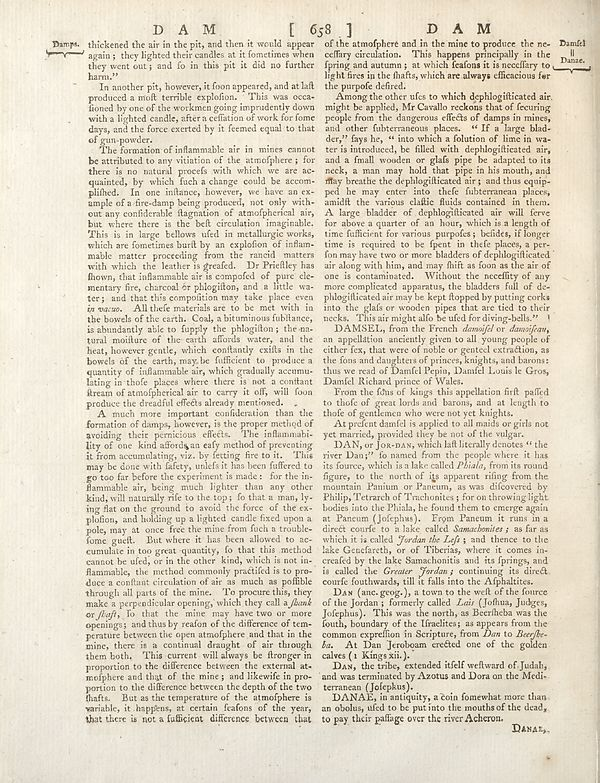
\includegraphics[width=0.85\textwidth]{../scans/page-1214-17d180a99e0a.jpg}
\caption*{Source scan: \texttt{page-1214-17d180a99e0a.jpg}}
\end{figure}

\end{document}
